\documentclass[letterpaper,journal]{IEEEtran}
\usepackage{amsmath,amsfonts}
\usepackage{algorithmic}
\usepackage{algorithm}
\usepackage{array}
\usepackage[caption=false,font=normalsize,labelfont=sf,textfont=sf]{subfig}
\usepackage{textcomp}
\usepackage{stfloats}
\usepackage{url}
\def\UrlBreaks{\do\/\do\-\do\_}
\usepackage{verbatim}
\usepackage{graphicx}
\usepackage{cite}
\usepackage{multirow}
\usepackage{balance}
\hyphenation{op-tical net-works semi-conduc-tor IEEE-Xplore}

\begin{document}

\title{MultiEMiT: Multimodal Emotion, Irony, and Semiotic Relation Detection in Italian Social TV via Correlation Prompting}

\author{Andrea~Author,~\IEEEmembership{Graduate Student Member,~IEEE,}
        Co-Author~One,~\IEEEmembership{Member,~IEEE,}
        and~Co-Author~Two,~\IEEEmembership{Senior Member,~IEEE}%
\thanks{Manuscript received October 27, 2026. This work was conducted within the M.EMO.RAI collaboration between the Department of Computer Science, University of Turin, 10149 Turin, Italy, and the ICT Directorate of Rai (Radiotelevisione Italiana), Turin, Italy.}%
\thanks{Corresponding author: Andrea Author (e-mail: andrea.author@unito.it).}}

% The paper headers
\markboth{IEEE Transactions on Affective Computing,~Vol.~XX, No.~X, October~2026}%
{Author \MakeLowercase{\textit{et al.}}: MultiEMiT: Multimodal Affective Computing in Italian Social TV}

\maketitle

\begin{abstract}
During live television broadcasts, viewers react on social media with a blend of text, screengrabs, and memes. Decoding affective intent in this context is hard: posts are short, labels are heavily skewed, and images often twist or invert the written message. We present MultiEMiT, a multimodal dataset of Italian Social Media posts and comments annotated across five dimensions: fine-grained emotions under Plutchik's taxonomy, irony and sarcasm, hate speech, target orientation (broadcast content versus program container), and semiotic text--image relationships (additive, parallel, divergent). We evaluate task-specialized Encoders models (BERT and Vision Transformer) against an open-weights generative model, Pixtral 12B.  To exploit label dependencies, we introduce correlation prompting: directly injecting labels from other levels of annotation into the input text as support of the classification. Visual context improves multi-label emotion recognition, lifting Macro $F_1$ by $+13$\% over text-only models. In irony detection, raw visual features introduce semantic noise and degrade performance through the modality gap; injecting correlation priors resolves this misalignment and pushes Dual-Encoder accuracy to $F_1 = 0.740$. Across all tasks, lightweight discriminative models outperform the fine-tuned 12-billion-parameter foundation model.
\end{abstract}

\begin{IEEEkeywords}
Affective computing, emotion detection, irony detection, multimodal fusion, Social TV, correlation prompting, vision-language models, Italian NLP.
\end{IEEEkeywords}

\section{Introduction}
\IEEEPARstart{T}{elevision} audiences no longer watch broadcasts in silence. During live debates, political talk shows, and reality competitions, viewers actively turn to second-screen platforms like Twitter to share commentary, memes, and screenshots \cite{SocialTV}. This stream of real-time viewer feedback offers broadcasters far richer signals than traditional audience ratings, providing immediate insight into public controversy, approval, and emotional engagement \cite{memorai}. 

Capturing these affective signals computationally, however, presents severe challenges. Social TV commentary is short, colloquial, and inherently multimodal. Viewers attach screengrabs and reaction images that do not merely mirror the written text; they exaggerate emotional tone, introduce sarcasm, or invert the literal message completely. 

The foundational question that motivated this investigation is: \textit{how much do attached images genuinely contribute to identifying human affective intent in multimodal social network posts?} During the manual annotation of our dataset, we observed a crucial empirical phenomenon: human annotator agreement increased substantially when annotators were provided with the attached images compared to reading the text alone. Visual context anchored ambiguous social commentary, establishing consensus where text alone yielded divergent interpretations. This observation directly motivates our central research hypothesis: \textit{does this visual grounding similarly carry over to neural models, or do visual features introduce semantic noise when discourse turns non-literal?}

Furthermore, while multilingual initiatives have advanced text-based emotion analysis, computational resources for Italian remain scarce, and existing benchmarks focus exclusively on unimodal text \cite{bianchi2021feel, emit, MultiEmotion}. To bridge this gap, we introduce \textbf{MultiEMiT}, a multimodal dataset of Italian Twitter commentary gathered from television broadcasts. MultiEMiT provides annotations across five pragmatic layers: fine-grained emotions under Plutchik's taxonomy \cite{Plutchik}, irony and sarcasm, offensiveness, target orientation (program container versus broadcast content), and semiotic text-image relationships \cite{MultiM}. Our benchmarking focuses on three primary classification tasks: Emotion Detection, Irony Detection, and Semiotic Relation Detection, with offensiveness and target serving as contextual signals. To expand training coverage for baseline text encoders, we also draw on the external unimodal EMiT (for Emotions) \cite{emit} and IronITA (for Irony) \cite{ironita2018} corpora.

An in-depth statistical analysis of MultiEMiT's multi-layered annotations revealed another compelling pattern: extensive empirical co-occurrences connect different annotation levels. For instance, irony correlates with joy, sarcasm pairs strongly with disgust and offensiveness, and program-directed commentary associates with viewer trust. Rather than treating these dimensions as isolated tasks or leaving neural models blind to these structural dependencies, we investigated whether artificial models could actively benefit from these cross-layer co-occurrences. To this end, we propose \textbf{Correlation Prompting}, a strategy that converts empirical Pearson correlation statistics directly into natural language prompt prefixes, providing explicit inductive priors during training and inference.

To evaluate these hypotheses systematically, we frame our study around three core research questions:
\begin{itemize}
    \item \textbf{RQ1 (Visual Context):} Does adding visual context help neural models detect emotion and irony, or do images introduce distracting noise in the classification of posts?
    \item \textbf{RQ2 (Correlation Prompting):} Does injecting statistical label correlations directly into text inputs improve accuracy across discriminative and generative architectures?
    \item \textbf{RQ3 (Architectural Paradigms):} How do compact, task-specialized discriminative models (BERT-ViT Dual-Encoders with Classifier Chains) compare with a 12 billion parameter foundation model (Pixtral 12B)?
\end{itemize}

The main contributions of this work are summarized as follows:
\begin{itemize}
    \item We introduce \textbf{MultiEMiT}, the first multi-layered multimodal dataset of Italian Social TV commentary, pairing text with broadcast media and reaction memes across five pragmatic dimensions.
    \item We empirically demonstrate the divergent impact of visual grounding across literal and figurative discourse: while images resolve textual ambiguity in emotion recognition, unguided visual features introduce semantic dissonance in irony detection.
    \item We propose \textbf{Correlation Prompting}, demonstrating that injecting multi-level statistical dependencies into model prompts effectively bridges cross-modal conflict and yields substantial performance gains.
    \item We present a rigorous comparative benchmark evaluating compact Dual-Encoders against the 12B parameter Pixtral model, identifying key failure modes such as exposure bias and hallucination loops in generative affective classification.
\end{itemize}

The rest of this paper is organized as follows. Section~\ref{sec:related_works} situates MultiEMiT within Italian affective computing, Social TV analytics, and multimodal document intent. Section~\ref{sec:dataset_analysis} describes the corpus collection, annotation protocol, and cross-dimensional correlations. Section~\ref{sec:experimental_design} defines our classification tasks, Dual-Encoder architecture, correlation prompting strategy, and Pixtral configurations. Section~\ref{sec:results} presents comparative evaluations and subset analyses across semiotic relations. Section~\ref{sec:conclusion} summarizes our findings and directions for future work.

\section{Related Works}
\label{sec:related_works}

Most annotated resources for affective computing focus on English. While multilingual initiatives like BRIGHTER \cite{brighter_project} aggregate emotion data across 28 languages and 100,000 instances, they omit Italian, pointing users toward standalone external sets like FEEL-IT \cite{bianchi2021feel}. This gap leaves Italian social media underrepresented in multi-label benchmarks, despite distinct cultural and linguistic norms in regional political discourse.

Early Italian resources focused strictly on binary or three-class polarity. The first dedicated shift toward fine-grained categories came with \textit{FEEL-IT} \cite{bianchi2021feel}, which collected 2,037 tweets across politics, sports, and healthcare during 2020. Annotated with Ekman's four basic emotions (anger, joy, sadness, fear), FEEL-IT established that Italian language models like UmBERTo \cite{musixmatch-2020-umberto} produce reliable affective classifiers. Yet a four-class schema misses mixed feelings and conversational nuances common in viewer reactions. To address broader emotional ranges, \textit{MultiEmotions-It} \cite{MultiEmotion} annotated YouTube and Facebook comments across Plutchik's eight primary emotions \cite{Plutchik}, polarity, and sarcasm. Their findings showed that while polarity models perform consistently, multi-label emotion recognition and sarcasm detection suffer from severe class sparsity and label ambiguity.

Second-screen platforms have changed how broadcasters analyze viewer engagement \cite{SocialTV}. Traditional television ratings (like Auditel) measure raw viewer counts; they cannot gauge whether an audience is laughing, outraged, or sympathetic. The \textit{M.EMO.RAI} project was formed to address this limitation, establishing a joint partnership between the University of Turin and Rai (Radiotelevisione Italiana) \cite{memorai}. The goal was an automated system to track audience reactions during live broadcasts by ingesting public social network commentary.

This partnership led to the \textit{EMiT} (Emotions in Italian) corpus, benchmarked as an EVALITA 2023 shared task \cite{emit}. With 5,966 social media posts from live broadcasts (including the Sanremo Festival and scripted drama), EMiT adopted Plutchik's taxonomy. It also introduced the \textit{Target} dimension, distinguishing whether a comment attacks the broadcast \textit{Content} (the topic, guest, or political issue) or evaluates the \textit{Container} (the host, studio format, or network production). EVALITA benchmark results showed that while classifiers perform well on familiar shows, accuracy drops on out-of-domain broadcasts. We use EMiT as an external textual corpus to pre-train and enrich our baseline emotion encoders.

Irony detection requires models to recognize when a speaker's intended meaning opposes their literal words. In Italian NLP, the standard benchmark is \textit{IronITA} \cite{ironita2018}, curated for EVALITA 2018 with nearly 5,000 tweets annotated for irony and sarcasm (defined as hostile or denigratory mockery). Results on IronITA showed that text-only classifiers struggle on short posts when pragmatic context is missing. To provide our models with domain-adapted pragmatic competence, we use IronITA to fine-tune UmBERTo before evaluating on television commentary.

Linguistic text only tells half the story in modern social media. In their study on document intent, Kruk et al. \cite{MultiM} demonstrated that images in social posts rarely just illustrate captions; they alter communicative intent through distinct semiotic relationships, ranging from complementary addition to direct divergence. Incongruent or divergent pairings generate satirical humor and memes, where the image subverts the text. Kruk et al. studied English Instagram posts. The semiotic relationship between text and visual media in Italian political satire and reality television remains largely unstudied. MultiEMiT applies this semiotic framework directly to Italian Social TV.

\section{Dataset Analysis}
\label{sec:dataset_analysis}

We introduce the MultiEMiT corpus, a multi-layered multimodal dataset of Italian Twitter commentary gathered during live television broadcasts. The data originates from the M.EMO.RAI project \cite{memorai}, which set out to track audience emotional responses in real time. Rather than restricting annotations to positive or negative sentiment, MultiEMiT applies an expanded eight-emotion taxonomy derived from Plutchik's psychoevolutionary model \cite{Plutchik}.

MultiEMiT draws from two television broadcasts representing contrasting formats and registers:

\textit{ProSAT:} Twitter commentary on \textit{Propaganda Live}, a satirical talk show on LA7 combining investigative journalism and political commentary \cite{propagandalive}. The collection captures the broadcast of November 19, 2021, when host Diego Bianchi reported live from the Poland--Belarus border during a humanitarian crisis. The gravity of the event prompted solemn reactions dominated by indignation, grief, and civic debate.

\textit{EMiT (Pechino Express):} Collected as an extension of the EVALITA EMiT benchmark \cite{emit}, this sub-corpus covers \textit{Pechino Express}, an adventure reality show broadcast on Rai2 \cite{pechinoexpress}. Collected during the season premiere on February 11, 2020, viewer discourse centers on lighthearted entertainment, contestant rivalries, and humorous commentary.

Both partitions share an identical structure: a purely textual partition and a multimodal partition pairing the text with its attached media (screenshots, edited images, and memes). This paired structure allows direct comparison between unimodal and multimodal models, showing where visual content modulates the written post. In addition to MultiEMiT, we use the external textual EMiT corpus (5,966 posts across multiple programs \cite{emit}) as supplementary training data for baseline emotion encoders.

Annotation was conducted on Sensitag, a web annotation platform developed at the University of Turin. Each post was evaluated independently by three annotators with backgrounds in computer science or linguistics. Final labels were assigned by majority vote (at least two out of three annotators agreeing).

The corpus is annotated across five pragmatic dimensions:
\begin{itemize}
    \item \textbf{Emotions:} Ten affective categories based on Plutchik's model \cite{Plutchik} (\textit{Joy}--\textit{Sadness}, \textit{Trust}--\textit{Disgust}, \textit{Fear}--\textit{Anger}, \textit{Surprise}--\textit{Anticipation}), supplemented with \textit{Love} and \textit{Neutral}. This task is multi-label, allowing posts to carry multiple concurrent emotional states.
    \item \textbf{Irony and Sarcasm:} Three exclusive classes separating literal statements (\textit{Unironic}), humorous figurative inversion (\textit{Irony}), and hostile, denigratory mockery (\textit{Sarcasm}).
    \item \textbf{Hate Speech:} Identifies abusive language, insults, or harassment directed at individuals or protected groups.
    \item \textbf{Target:} Distinguishes whether comments address the broadcast \textit{Content} (political issues, guests, or news events) or the \textit{Container} (the studio host, network, or production execution).
    \item \textbf{Semiotic Relation:} Categorizes multimodal document intent \cite{MultiM} into \textit{Additive} (modality enrichment), \textit{Parallel} (redundant information), and \textit{Divergent} (ironic contrast or meme dissonance).
\end{itemize}

Sarcasm and emotion in short social media posts are inherently ambiguous. Read in isolation, a comment on the border crisis such as \textit{``Terrible, I am ashamed to be European''} could be seen as shame (\textit{Disgust} + \textit{Fear}), contempt (\textit{Anger} + \textit{Disgust}), or disapproval (\textit{Surprise} + \textit{Sadness}).

Providing annotators with the attached image resolved much of this ambiguity, substantially lifting inter-annotator agreement (Fleiss' $\kappa$) across most emotion labels. Seeing photos of shivering refugees grounded the context, directing consensus toward sadness and distress. This empirical finding provides direct justification for multimodal modeling: if visual context clarifies ambiguous intent for human annotators, multimodal neural architectures should benefit from the same disambiguating cues.

Following gold-standard consolidation, the MultiEMiT corpus resulted in two main partitions: a purely \textbf{Textual} dataset comprising 2,909 posts, and a \textbf{Multimodal} dataset comprising 645 posts with paired image attachments. 

As typical of social media discourse, label distributions exhibit pronounced class imbalance. Tables~\ref{table:text_dist} and~\ref{table:multi_dist} present the complete distribution of labels across both partitions, broken down by broadcast sub-corpus.

\begin{table}[!t]
\centering
\caption{Label Distribution in the MultiEMiT Textual Dataset (2,909 Posts)}
\label{table:text_dist}
\begin{tabular}{l c c c}
\hline
\textbf{Label} & \textbf{Total (2,909)} & \textbf{ProSAT} & \textbf{EMiT} \\
\hline
\multicolumn{4}{l}{\textit{Emotions (multi-label)}} \\
\hline
Love & 340 & 119 & 221 \\
Anticipation & 201 & 75 & 126 \\
Disgust & 410 & 207 & 203 \\
Trust & 613 & 281 & 332 \\
Joy & 552 & 257 & 295 \\
Neutral & 321 & 31 & 290 \\
Fear & 55 & 44 & 11 \\
Anger & 163 & 121 & 42 \\
Surprise & 486 & 225 & 261 \\
Sadness & 255 & 211 & 44 \\
\hline
\multicolumn{4}{l}{\textit{Irony}} \\
\hline
Irony & 481 & 237 & 244 \\
Unironic & 2,072 & 828 & 1,244 \\
Sarcasm & 41 & 15 & 26 \\
\hline
\multicolumn{4}{l}{\textit{Offensiveness}} \\
\hline
Offensive & 52 & 31 & 21 \\
\hline
\multicolumn{4}{l}{\textit{Target}} \\
\hline
Container & 1,147 & 343 & 804 \\
Content & 1,138 & 710 & 428 \\
\hline
\end{tabular}
\end{table}

\begin{table}[!t]
\centering
\caption{Label Distribution in the MultiEMiT Multimodal Dataset (645 Posts)}
\label{table:multi_dist}
\begin{tabular}{l c c c}
\hline
\textbf{Label} & \textbf{Total (645)} & \textbf{ProSAT} & \textbf{EMiT} \\
\hline
\multicolumn{4}{l}{\textit{Emotions (multi-label)}} \\
\hline
Love & 50 & 17 & 33 \\
Anticipation & 61 & 10 & 51 \\
Disgust & 78 & 18 & 60 \\
Trust & 214 & 82 & 132 \\
Joy & 168 & 79 & 89 \\
Neutral & 90 & 21 & 69 \\
Fear & 4 & 4 & 0 \\
Anger & 34 & 29 & 5 \\
Surprise & 82 & 24 & 58 \\
Sadness & 25 & 23 & 2 \\
\hline
\multicolumn{4}{l}{\textit{Irony}} \\
\hline
Irony & 109 & 21 & 88 \\
Unironic & 516 & 199 & 317 \\
Sarcasm & 20 & 5 & 15 \\
\hline
\multicolumn{4}{l}{\textit{Offensiveness}} \\
\hline
Offensive & 6 & 3 & 3 \\
\hline
\multicolumn{4}{l}{\textit{Target}} \\
\hline
Container & 395 & 103 & 292 \\
Content & 199 & 85 & 114 \\
\hline
\multicolumn{4}{l}{\textit{Semiotic Relation}} \\
\hline
Additive & 389 & 158 & 231 \\
Divergent & 158 & 42 & 116 \\
Parallel & 100 & 10 & 90 \\
\hline
\end{tabular}
\end{table}

Across both partitions, the most frequent affective states are \textit{Trust} and \textit{Joy}, indicating an overall positive engagement with broadcast programming. However, negative emotions exhibit marked domain dependency: \textit{Sadness}, \textit{Anger}, and \textit{Fear} are heavily concentrated within ProSAT due to the geopolitical reportage, whereas they remain negligible in the lighthearted Pechino Express subset.

Similarly, irony displays genre-specific dynamics. In the multimodal corpus, irony is prevalent in Pechino Express (88 instances) despite Propaganda Live being a satirical format. This occurs because the specific Propaganda Live episode under study addressed an acute humanitarian crisis, prompting solemn reflection rather than playful sarcasm. Regarding semiotic relations, the \textit{Additive} relation dominates in both subsets, while \textit{Parallel} and \textit{Divergent} relations appear far more frequently in entertainment contexts where visual memes thrive.

\begin{figure*}[!t]
\centering
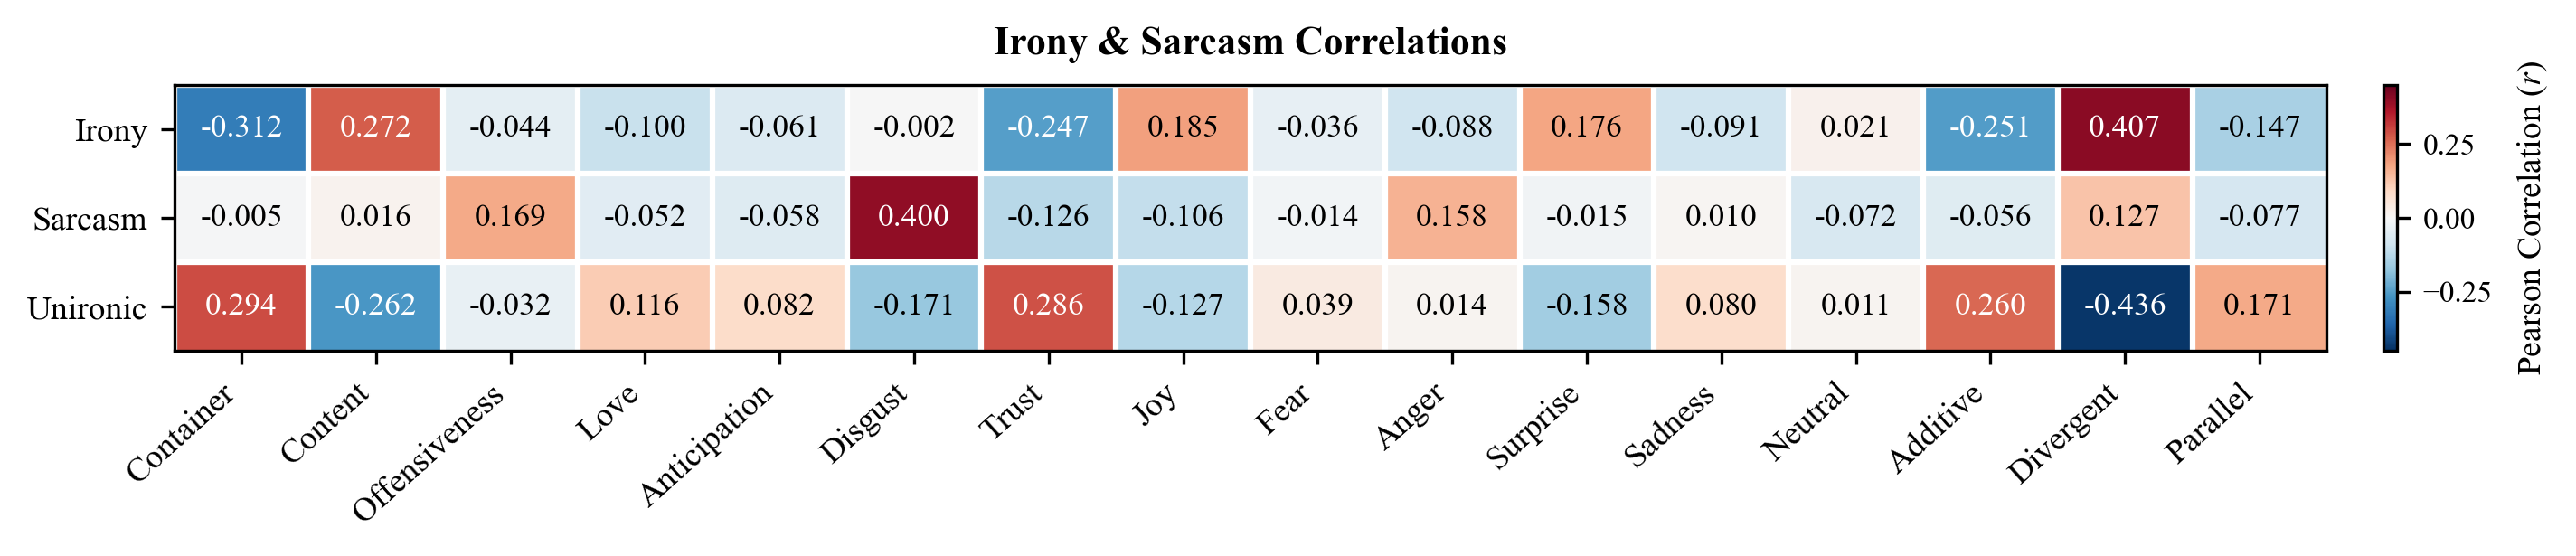
\includegraphics[width=\textwidth]{imgs/irony_correlations_english.png}
\caption{Pearson correlation matrix for the irony and sarcasm dimension across multi-level annotations.}
\label{fig:irony_correlations}
\end{figure*}

\begin{figure*}[!t]
\centering
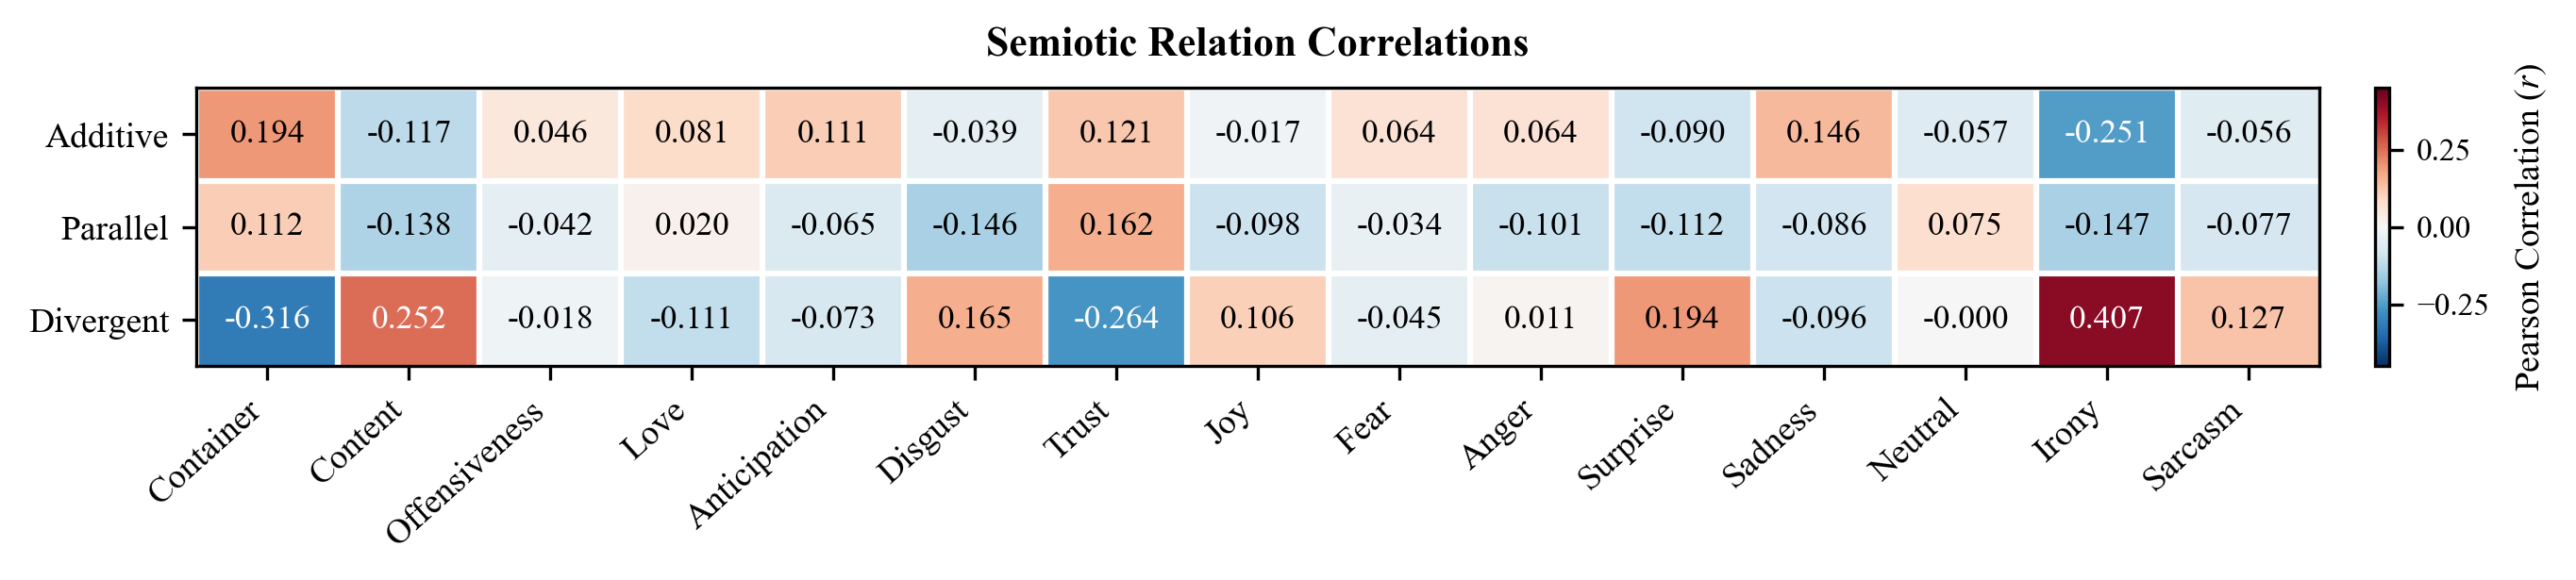
\includegraphics[width=\textwidth]{imgs/relation_correlations_english.png}
\caption{Pearson correlation matrix for semiotic text--image relations against contextual and affective markers.}
\label{fig:relations_correlations}
\end{figure*}

The multi-layered annotation of MultiEMiT enables systematic investigation into the statistical dependencies connecting emotional, figurative, and semiotic dimensions. By computing Pearson correlation coefficients ($r$) across all label pairs, we identified pronounced interdependencies indicating that pragmatic categories act as strong mutual predictors.

\begin{figure}[!t]
\centering
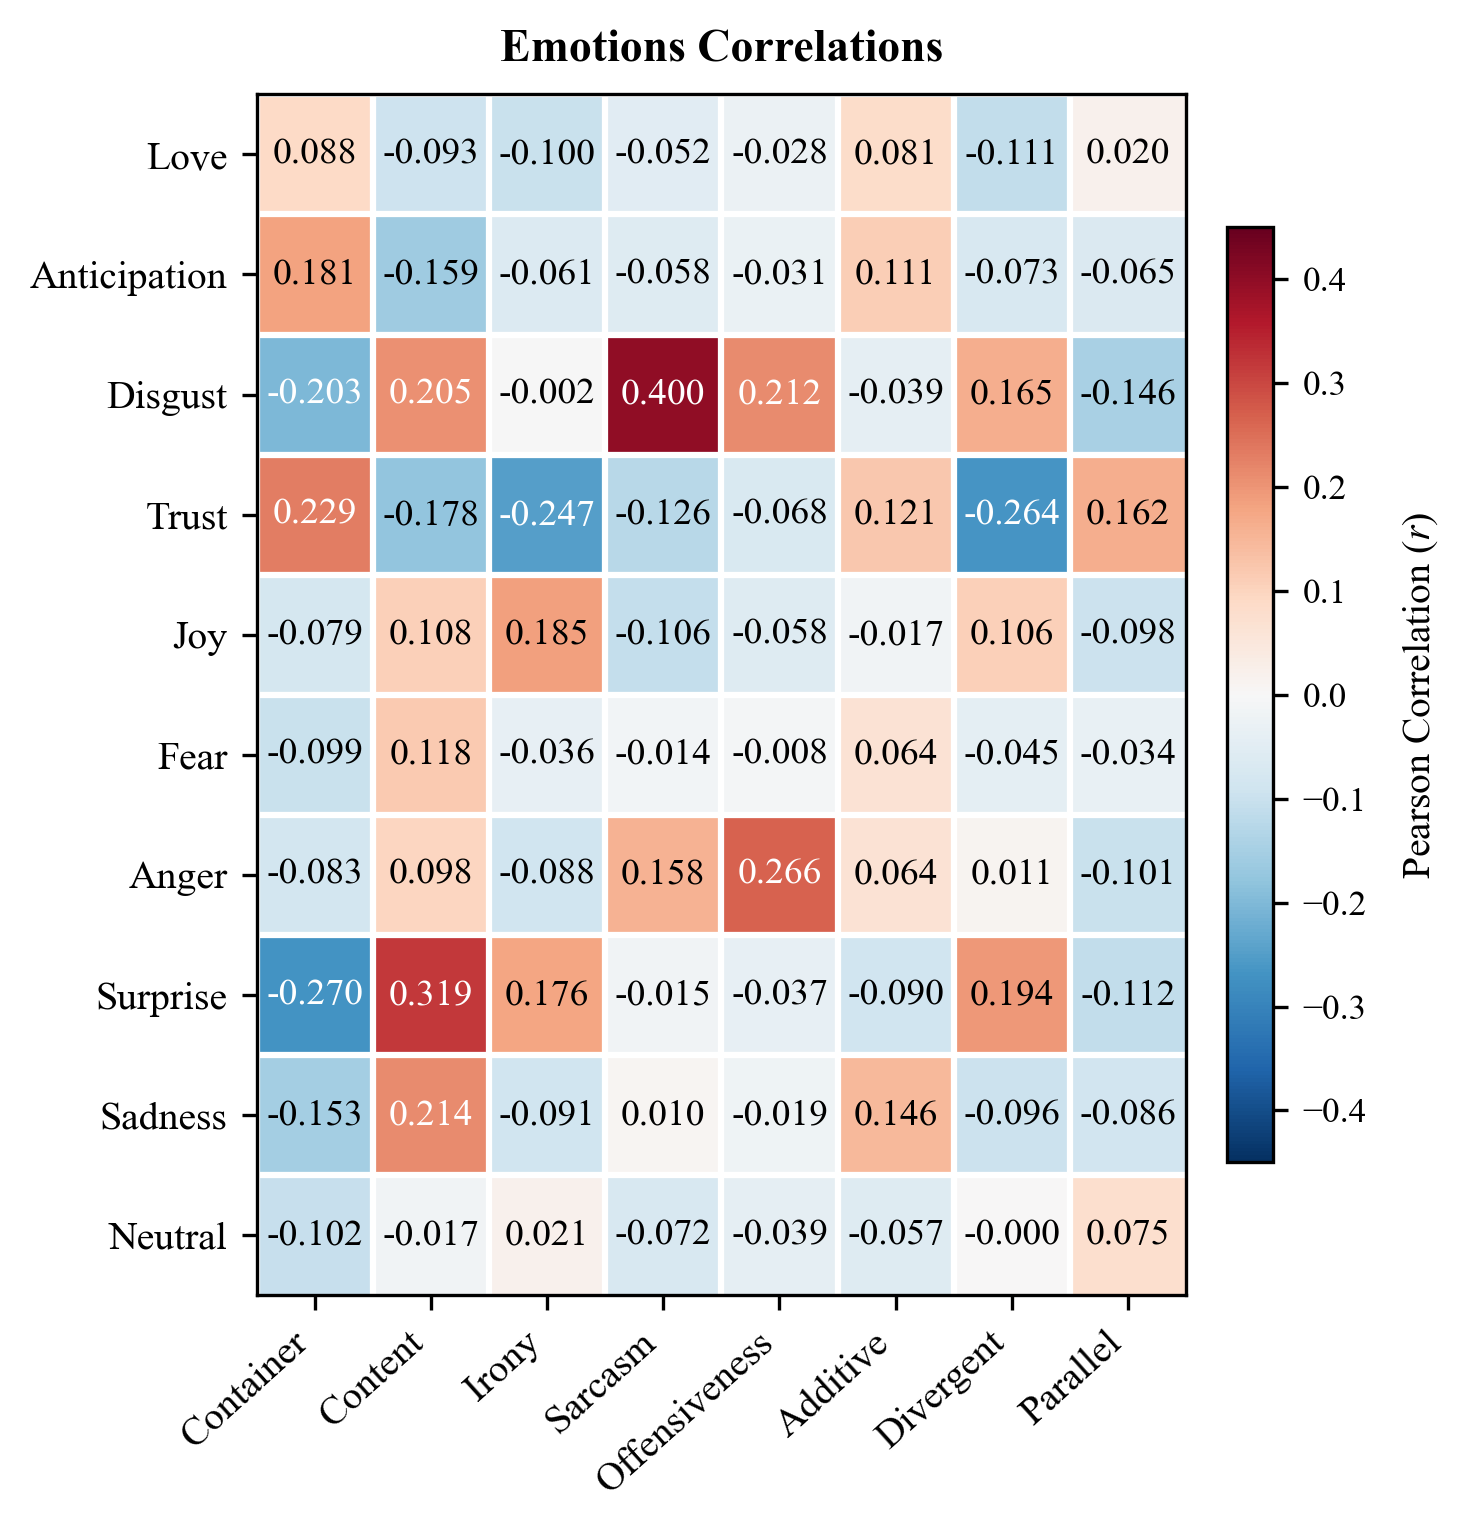
\includegraphics[width=0.92\columnwidth]{imgs/emotion_correlations_english.png}
\caption{Emotions Correlations: Pearson correlation matrix between emotion labels and contextual dimensions (broadcast targets, figurative speech, and semiotic relations).}
\label{fig:emotions_correlations}
\end{figure}

Examining the correlation matrix for \textbf{Emotions} (Fig.~\ref{fig:emotions_correlations}), a clear dichotomy emerges between the \textit{Container} and \textit{Content} targets. Program-directed affective states (\textit{Trust} $r = 0.229$, \textit{Anticipation} $r = 0.181$) correlate positively with Container, indicating audience loyalty toward the show. Conversely, content-reactive emotions (\textit{Surprise} $r = 0.319$, \textit{Sadness} $r = 0.214$, \textit{Disgust} $r = 0.205$) associate with Content. Sarcasm also reveals a hostile pragmatic pattern, correlating positively with \textit{Disgust} ($r = 0.400$), \textit{Anger} ($r = 0.158$), and offensive language ($r = 0.212$).

Analyzing \textbf{Irony} (Fig.~\ref{fig:irony_correlations}), we observe that figurative speech relies fundamentally on semiotic contrast. Irony correlates strongly with \textit{Divergent} text--image relations ($r = 0.407$) and the \textit{Content} target ($r = 0.272$), demonstrating that multimodal irony frequently arises from intentional tension between the visual image and the written caption. Sincere posts (\textit{Unironic}), by contrast, correlate with \textit{Container} ($r = 0.294$), \textit{Trust} ($r = 0.286$), and complementary visual relations (\textit{Additive} $r = 0.260$, \textit{Parallel} $r = 0.171$).

Semiotic relations (Fig.~\ref{fig:relations_correlations}) confirm that divergent pairings drive social media irony: Divergent posts correlate positively with \textit{Irony} ($r = 0.407$), \textit{Content} ($r = 0.252$), and \textit{Surprise} ($r = 0.194$). In contrast, the \textit{Additive} relation associates with \textit{Container} ($r = 0.194$) and narrative elaboration, while the \textit{Parallel} relation exhibits minimal correlation with complex emotional states, reflecting literal and redundant text--image usage.

\section{Experimental Design}
\label{sec:experimental_design}

\begin{figure*}[!t]
\centering
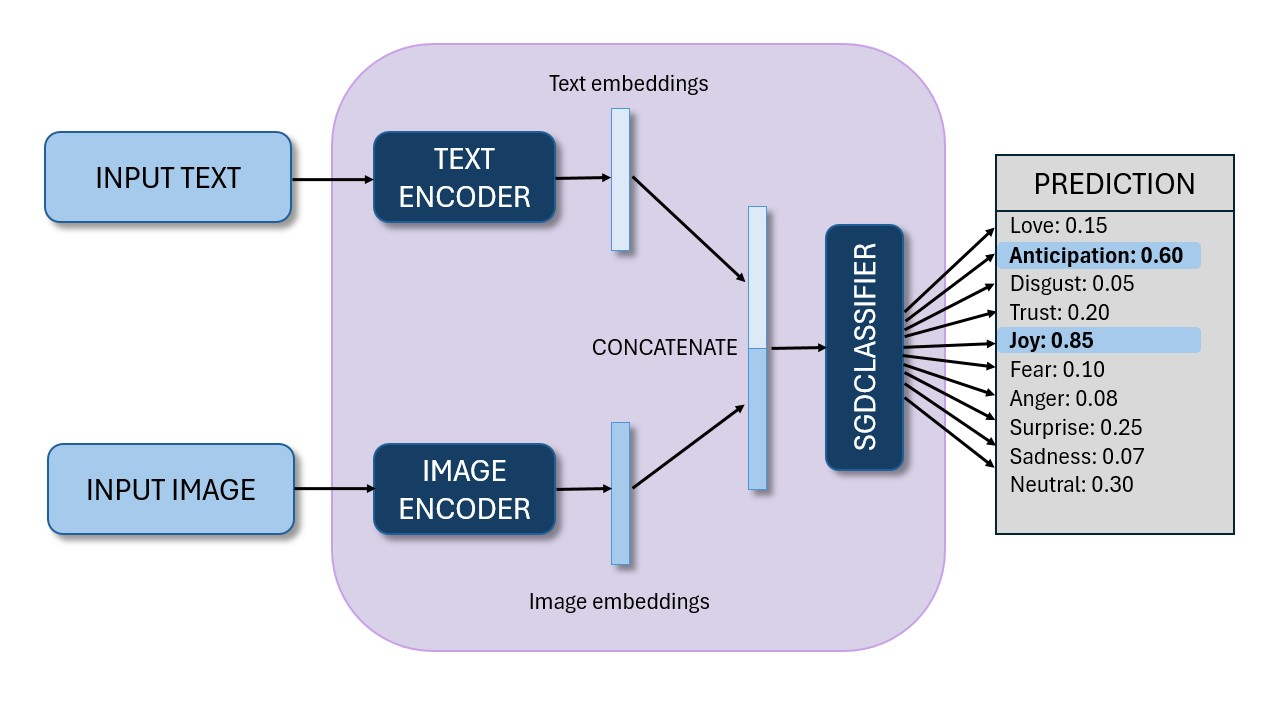
\includegraphics[width=0.78\textwidth]{imgs/model_architecture.jpeg}
\caption{Dual-Encoder multimodal architecture. Text and image representations are extracted in parallel via domain-adapted BERT and ViT encoders, concatenated into a joint vector ($d=1536$), and passed to a Classifier Chain head.}
\label{fig:dual_encoder_arch}
\end{figure*}

This section details the experimental methodology established to evaluate affective classification on the MultiEMiT corpus. We evaluate three distinct tasks: Emotion Detection, Irony Detection, and Semiotic Relation Detection. The experiments measure the performance differences between unimodal textual baselines, a discriminative multimodal architecture (Dual-Encoder), and a generative foundation model (Pixtral 12B), while assessing the empirical impact of correlation prompting across architectures.

We formalize three classification benchmarks corresponding to different levels of communicative intent:
\begin{itemize}\setlength{\itemsep}{1pt}\setlength{\parskip}{0pt}\setlength{\topsep}{2pt}
    \item \textbf{Emotion Detection:} Multi-label classification over ten candidate emotions (\textit{Anger}, \textit{Anticipation}, \textit{Disgust}, \textit{Fear}, \textit{Joy}, \textit{Love}, \textit{Neutral}, \textit{Sadness}, \textit{Surprise}, and \textit{Trust}). Models predict any valid subset of concurrent emotions using binary cross-entropy or binary chains.
    \item \textbf{Irony Detection:} Single-label classification categorizing each post into one of three mutually exclusive classes: \textit{Unironic}, \textit{Irony}, or \textit{Sarcasm}.
    \item \textbf{Semiotic Relation Detection:} Single-label classification identifying the semantic text--image interaction as \textit{Additive}, \textit{Parallel}, or \textit{Divergent}.
\end{itemize}

Due to heavy class skew, raw accuracy paints a misleading picture of model quality. We therefore evaluate systems using \textbf{Precision}, \textbf{Recall}, and the \textbf{F1-score}. In overall comparisons across all three tasks, the \textbf{Macro F1-score} serves as the primary metric, weighting each class equally to penalize poor performance on minority labels. In fine-grained subset evaluations across semiotic relations (Section~\ref{sec:results}), we report the \textbf{Micro F1-score} to maintain metric stability when sample sizes in individual subsets are small.

To establish strong text-only reference points, we evaluated models built on the RoBERTa architecture. For Irony and Semiotic Relation detection, we used \textit{UmBERTo} \cite{musixmatch-2020-umberto}, a RoBERTa-based language model pre-trained on Italian Common Crawl with whole-word masking. For Irony detection, UmBERTo was first fine-tuned on the IronITA benchmark \cite{ironita2018} before adaptation to MultiEMiT. For Emotion Detection, we used \textit{FEEL-IT} \cite{bianchi2021feel}, fine-tuned on the combined MultiEMiT textual split and the external EMiT dataset \cite{emit} to adapt its representation space to our ten-class taxonomy. These text models process the tweet text alone without visual inputs.

To capture cross-modal interactions, we implemented a discriminative Dual-Encoder pipeline (Fig.~\ref{fig:dual_encoder_arch}). 
The textual modality is processed by the domain-adapted language encoder (FEEL-IT for emotions, UmBERTo for irony and relations), while the visual modality is processed in parallel by a Vision Transformer (ViT-base-patch16-224) \cite{dosovitskiy2021vit}.
Both unimodal encoders extract high-level representations: the 768-dimensional `[CLS]` token embedding from the text transformer and the 768-dimensional pooled representation from the ViT are concatenated into a 1536-dimensional joint multimodal vector.

To predict class labels from this joint representation, we employ Classifier Chains \cite{pedregosa2011scikit}. This architecture models label interdependencies by sequentially conditioning subsequent binary classifiers on previous predictions, making it well suited for multi-label emotion spaces. Specifically, we configure Scikit-Learn's \texttt{ClassifierChain} wrapping an \texttt{SGDClassifier} with logistic loss, $L_2$ regularization, and fixed random seeding. This linear head projects the concatenated latent space to class predictions without overfitting on the compact multimodal split.

Motivated by the strong label dependencies discovered during corpus analysis (Section~\ref{sec:dataset_analysis}), we developed a structured \textit{Correlation Prompting} strategy. Rather than hoping the neural network will infer subtle cross-task correlations from scarce training examples, we inject empirical Pearson correlation coefficients directly into the input text as natural language context. For example, in the Irony detection task, the input tweet is appended with: \textit{``Statistics: Sarcasm correlates positively with Disgust and Anger. Irony correlates positively with Divergent relation.''}

To evaluate model sensitivity to the volume of injected priors, we structured prompts across three distinct correlation tiers based on Pearson coefficient thresholds: (i) \textbf{Short prompts}, incorporating only strong associations with $|r| \ge 0.25$; (ii) \textbf{Medium prompts}, including moderate correlations with $|r| \ge 0.20$; and (iii) \textbf{Long prompts}, providing detailed contextual priors with all correlations satisfying $|r| \ge 0.15$. All prompt instructions were formulated in English, following findings from the BRIGHTER benchmark \cite{brighter_project} indicating that multilingual LLMs adhere better to instructions and exhibit lower variance when prompted in English rather than the target language.

To compare specialized discriminative systems against modern generative vision-language models, we benchmarked \textbf{Pixtral 12B} \cite{pixtral}, an open-weights multimodal language model based on Mistral Nemo featuring a dedicated 400M-parameter vision encoder capable of handling arbitrary image resolutions.
We evaluated Pixtral across three experimental regimes:
\begin{itemize}\setlength{\itemsep}{1pt}\setlength{\parskip}{0pt}\setlength{\topsep}{2pt}
    \item \textbf{Zero-Shot Prompting:} Out-of-the-box reasoning across prompt tiers (Short, Medium, and three Long prompt formulations: \textit{long\_v1}, \textit{long\_v2}, \textit{long\_v3}), testing generation with and without correlation context.
    \item \textbf{Few-Shot (Three-Shot) Prompting:} In-context learning for Semiotic Relation Detection, providing three complete multimodal exemplars (one per relation category) within the prompt window.
    \item \textbf{LoRA Fine-Tuning:} Low-Rank Adaptation on the MultiEMiT multimodal training set ($r=16$, $\alpha=32$, RSLoRA, all linear target modules, dropout $0.1$). This configuration adapts 66,322,432 parameters out of 12.75 billion (0.52\% trainable parameters). Training ran with per-device batch size 1, 8 gradient accumulation steps (effective batch size 8), learning rate $3 \times 10^{-5}$, FP16 mixed precision, and gradient checkpointing over 2 epochs.
\end{itemize}

All generative experiments were evaluated over three independent runs at two decoding temperatures: $T=0.1$ (greedy, low-variance decoding) and $T=0.9$ (stochastic exploratory decoding).

Unlike discriminative encoders that output bounded probability vectors over predefined classes, Pixtral generates labels autoregressively. During multi-label emotion fine-tuning, ranking bias and exposure bias degraded the stopping token (\texttt{<EOS>}), causing repetitive token loops and out-of-vocabulary synonyms (e.g., generating \textit{Joy, Joy, Happiness} instead of \textit{Joy}). To resolve this without retraining, we implemented a post-processing truncation parameter $n$, restricting extraction to the first $n$ unique valid taxonomy emotions generated. Setting $n=2$ matches the empirical ground truth and eliminates unconstrained tail hallucinations.

\section{Results and Discussion}
\label{sec:results}

This section presents the empirical evaluation of the unimodal and multimodal architectures across the three tasks: Emotion Detection, Irony Detection, and Semiotic Relation Detection. We analyze the quantitative impact of integrating visual features (comparing blind text baselines to the Dual-Encoder), the performance gains induced by correlation prompting, and the strengths and failure modes of Pixtral 12B. We also examine model behavior disaggregated across semiotic relational subsets.

Emotion detection represents the most challenging benchmark due to the high cardinality of the ten-class label space and the multi-label nature of affective expression in social media.

On the textual dataset, the baseline discriminative model (FEEL-IT fine-tuned on MultiEMiT and EMiT) achieved a Macro $F_1$-score of 0.460, increasing to 0.540 when trained with correlation prompting, and reaching 0.590 when retrained across two isolated phases with correlation context. When evaluating exclusively on the multimodal test set, the blind text-only baseline (evaluating only the text of multimodal posts) achieves a Macro $F_1$-score of 0.300 without correlations and 0.370 with correlations.

Introducing visual features via the Dual-Encoder architecture substantially enhances classification performance: the multimodal system achieves a Macro $F_1$-score of 0.430 without correlations and 0.450 with correlations. This marked improvement (+13\% absolute over the blind unprompted text baseline) empirically confirms that visual context provides essential disambiguating cues for recognizing emotional expressions in social commentary, with correlation prompting providing a complementary gain.

Turning to generative foundation models, fine-tuned Pixtral 12B achieved an $F_1$-score of 0.426 ($T=0.1$). While competitive with the discriminative Dual-Encoder without correlations (0.430), it remains below the correlation-prompted Dual-Encoder (0.450), showing that task-adapted discriminative representations remain superior for multi-label Italian emotion classification. Complete comparisons across prompt tiers and temperatures are reported in Table~\ref{tab:emotion_pixtral}.

\begin{table}[!t]
\centering
\caption{Complete Comparison: Pixtral 12B versus Dual-Encoder in Emotion Detection ($T=0.1$ and $T=0.9$)}
\label{tab:emotion_pixtral}
\footnotesize
\renewcommand{\arraystretch}{0.92}
\begin{tabular}{l l c c}
\hline
\textbf{Model} & \textbf{Configuration} & \textbf{T = 0.1 F1} & \textbf{T = 0.9 F1} \\
\hline
\multicolumn{4}{l}{\textit{Discriminative Multimodal (Dual-Encoder)}} \\
BERT-ViT & FT (With Corr.) & \textbf{0.450} & \textbf{0.450} \\
BERT-ViT & FT (No Corr.) & 0.430 & 0.430 \\
\hline
\multicolumn{4}{l}{\textit{Generative (Pixtral 12B)}} \\
Pixtral (long\_v1) & FT ($n=2$) & \textbf{0.426} & 0.359 \\
Pixtral (short) & FT ($n=2$) & 0.397 & \textbf{0.373} \\
Pixtral (short) & FT (all predictions) & 0.318 & 0.312 \\
Pixtral (short) & ZS (With Corr.) & 0.291 & 0.251 \\
Pixtral (long\_v1) & ZS (With Corr.) & 0.275 & 0.266 \\
Pixtral (medium) & ZS (With Corr.) & 0.269 & 0.262 \\
Pixtral (long\_v2) & ZS (No Corr.) & 0.266 & 0.237 \\
Pixtral (long\_v1) & ZS (No Corr.) & 0.261 & 0.261 \\
Pixtral (short) & ZS (No Corr.) & 0.261 & 0.291 \\
Pixtral (long\_v3) & ZS (With Corr.) & 0.258 & 0.262 \\
Pixtral (medium) & ZS (No Corr.) & 0.254 & 0.250 \\
Pixtral (long\_v2) & ZS (With Corr.) & 0.253 & 0.286 \\
Pixtral (long\_v1) & FT (all predictions) & 0.238 & 0.290 \\
Pixtral (long\_v3) & ZS (No Corr.) & 0.220 & 0.215 \\
\hline
\end{tabular}
\end{table}

\begin{table}[!t]
\centering
\caption{Impact of Truncation Parameter ($n$) on Pixtral Emotion Detection Performance}
\label{table:truncation_parameter}
\small
\begin{tabular}{c c}
\hline
\textbf{Number of Predictions ($n$)} & \textbf{Mean Macro F1} \\
\hline
1 & 0.338 \\
2 & \textbf{0.389} \\
3 & 0.339 \\
4 & 0.325 \\
5 & 0.308 \\
\hline
\end{tabular}
\end{table}

During Pixtral fine-tuning, autoregressive decoding generated repetitive loops and extra-taxonomical tokens when predicting emotion lists. However, qualitative analysis revealed that predicted emotions were ordered by descending model confidence. Implementing the truncation parameter $n$ to retain the top-$n$ unique valid emotions effectively eliminated generative noise. As detailed in Table~\ref{table:truncation_parameter}, performance peaks distinctly at $n=2$ (Mean Macro $F_1 = 0.389$). Allowing unconstrained generation ($n \ge 5$) degrades performance to 0.308, as spurious tail predictions incur heavy false-positive penalties. Setting $n=2$ matches the empirical ground truth, where the vast majority of posts express one or two concurrent emotions.

Disaggregating model performance across the Additive (ADD), Parallel (PAR), and Divergent (DIV) semiotic partitions reveals striking structural variations (Table~\ref{tab:subset_emotion}). 

\begin{table}[!t]
\centering
\caption{Emotion Detection Micro F1-score across Semiotic Subsets}
\label{tab:subset_emotion}
\small
\begin{tabular}{l c c c}
\hline
\textbf{Model Setting} & \textbf{ADD} & \textbf{PAR} & \textbf{DIV} \\
\hline
\multicolumn{4}{l}{\textit{Dual-Encoder (BERT--ViT)}} \\
No correlations & 0.47 & 0.52 & 0.38 \\
With correlations & \textbf{0.54} & \textbf{0.60} & 0.42 \\
\hline
\multicolumn{4}{l}{\textit{Generative LLM (Pixtral 12B)}} \\
Zero-Shot (No corr.) & 0.29 & 0.23 & \textbf{0.44} \\
Zero-Shot (With corr.) & 0.32 & 0.30 & 0.43 \\
Fine-tuned (No corr.) & 0.33 & 0.41 & 0.41 \\
\hline
\end{tabular}
\end{table}

Both model families experience their lowest scores on the \textit{Divergent} subset (Micro $F_1 = 0.38$ to $0.42$). In divergent posts, intentional tension between text and imagery disrupts emotional coherence, confounding automated classifiers. Conversely, models perform best on the \textit{Parallel} partition ($F_1 = 0.60$ for the prompted Dual-Encoder), where redundant visual information reinforces literal textual meaning. For the dominant \textit{Additive} subset, correlation prompting delivers a $+0.07$ boost for the Dual-Encoder, demonstrating that statistical priors help integrate complementary cross-modal evidence.

Irony detection presents an inverted dynamic compared to emotion recognition. In figurative discourse, visual content frequently introduces pragmatic incongruity rather than semantic convergence. Table~\ref{tab:irony_pixtral} summarizes comparative results.

\begin{table}[!t]
\centering
\caption{Complete Comparison: Pixtral 12B versus Dual-Encoder in Irony Detection ($T=0.1$ and $T=0.9$)}
\label{tab:irony_pixtral}
\footnotesize
\renewcommand{\arraystretch}{0.92}
\begin{tabular}{l l c c}
\hline
\textbf{Model} & \textbf{Configuration} & \textbf{T = 0.1 F1} & \textbf{T = 0.9 F1} \\
\hline
\multicolumn{4}{l}{\textit{Discriminative Multimodal (Dual-Encoder)}} \\
BERT-ViT & FT (With Corr.) & \textbf{0.740} & \textbf{0.740} \\
BERT-ViT & FT (No Corr.) & 0.630 & 0.630 \\
\hline
\multicolumn{4}{l}{\textit{Generative (Pixtral 12B)}} \\
Pixtral (long\_v2) & ZS (With Corr.) & \textbf{0.512} & 0.396 \\
Pixtral (long\_v2) & FT (all predictions) & 0.405 & \textbf{0.454} \\
Pixtral (short) & ZS (With Corr.) & 0.348 & 0.298 \\
Pixtral (long\_v3) & ZS (With Corr.) & 0.340 & 0.281 \\
Pixtral (short) & FT (all predictions) & 0.329 & 0.394 \\
Pixtral (medium) & ZS (With Corr.) & 0.264 & 0.270 \\
Pixtral (long\_v1) & ZS (With Corr.) & 0.248 & 0.295 \\
Pixtral (long\_v2) & ZS (No Corr.) & 0.165 & 0.218 \\
Pixtral (long\_v3) & ZS (No Corr.) & 0.148 & 0.198 \\
Pixtral (long\_v1) & ZS (No Corr.) & 0.126 & 0.158 \\
Pixtral (short) & ZS (No Corr.) & 0.054 & 0.108 \\
Pixtral (medium) & ZS (No Corr.) & 0.051 & 0.137 \\
\hline
\end{tabular}
\end{table}

When evaluated on the multimodal test set, the blind textual baseline achieves an $F_1$-score of 0.670 without correlations and 0.710 with correlations. In sharp contrast, the multimodal Dual-Encoder without correlations achieves an $F_1$-score of only 0.630, underperforming the blind text model by $-0.040$. This degradation points to a core multimodal challenge: unguided visual features act as semantic noise. Because irony relies on incongruity, raw visual embeddings pull the multimodal vector away from the textual signal. This pattern aligns with findings on the \textit{Modality Gap} \cite{liang2022mindgap}: concatenating representations from separately pre-trained encoders (UmBERTo and ViT) without joint cross-modal pre-training leaves a geometric misalignment in latent space.

Injecting statistical correlations reverses this drop: the correlation-prompted Dual-Encoder reaches an $F_1$-score of \textbf{0.740}, outperforming both the blind textual baseline (0.710) and unprompted multimodal fusion (0.630). Explicit priors help the classifier treat visual dissonance as evidence of irony rather than noise.

In the generative regime, Pixtral 12B struggles severely in zero-shot settings without correlations ($F_1$ ranging between 0.051 and 0.165 across prompt variants at $T=0.1$). However, incorporating correlation prompts triggers a dramatic recovery, elevating zero-shot performance to 0.512 with the \textit{long\_v2} prompt (+0.347 gain). After LoRA fine-tuning, Pixtral achieves an $F_1$-score of 0.454 ($T=0.9$). Although competitive, it remains substantially below the specialized Dual-Encoder (0.740).

Examining irony detection across semiotic subsets (Table~\ref{tab:subset_irony}) elucidates how models process multimodal dissonance.

\begin{table}[!t]
\centering
\caption{Irony Detection Micro F1-score across Semiotic Subsets}
\label{tab:subset_irony}
\small
\begin{tabular}{l c c c}
\hline
\textbf{Model Setting} & \textbf{ADD} & \textbf{PAR} & \textbf{DIV} \\
\hline
\multicolumn{4}{l}{\textit{Dual-Encoder (BERT--ViT)}} \\
No correlations & 0.83 & \textbf{1.00} & 0.55 \\
With correlations & \textbf{0.88} & \textbf{1.00} & \textbf{0.68} \\
\hline
\multicolumn{4}{l}{\textit{Generative LLM (Pixtral 12B)}} \\
Zero-Shot (No corr.) & 0.14 & 0.00 & 0.18 \\
Zero-Shot (With corr.) & 0.57 & 0.78 & 0.57 \\
Fine-tuned (No corr.) & 0.87 & \textbf{1.00} & 0.58 \\
\hline
\end{tabular}
\end{table}

On the \textit{Parallel} partition, both the Dual-Encoder and fine-tuned Pixtral achieve a perfect score of 1.00. This outcome arises because the gold multimodal test set contains zero ironic posts with a parallel relation; the trained models correctly classify all instances as sincere (\textit{Unironic}). Conversely, unprompted zero-shot Pixtral collapses on parallel instances (0.00), hallucinating false-positive irony. On the challenging \textit{Divergent} subset, where irony is concentrated, the Dual-Encoder without correlations attains only 0.55; injecting correlation prompting raises this to 0.68 (+0.13 gain), confirming that correlation priors are vital for decoding divergent visual irony.

Semiotic relation detection requires the model to directly categorize the semantic interaction between modalities into Additive, Parallel, or Divergent. Table~\ref{tab:relation_pixtral} presents the complete evaluation.

\begin{table}[!t]
\centering
\caption{Complete Comparison: Pixtral 12B versus Dual-Encoder in Semiotic Relation Detection ($T=0.1$ and $T=0.9$)}
\label{tab:relation_pixtral}
\footnotesize
\renewcommand{\arraystretch}{0.90}
\begin{tabular}{l l c c}
\hline
\textbf{Model} & \textbf{Configuration} & \textbf{T = 0.1 F1} & \textbf{T = 0.9 F1} \\
\hline
\multicolumn{4}{l}{\textit{Discriminative Multimodal (Dual-Encoder)}} \\
BERT-ViT & FT (With Corr.) & \textbf{0.690} & \textbf{0.690} \\
BERT-ViT & FT (No Corr.)  & 0.640 & 0.640 \\
\hline
\multicolumn{4}{l}{\textit{Generative (Pixtral 12B)}} \\
Pixtral (long\_v1) & FT (all predictions) & \textbf{0.613} & \textbf{0.574} \\
Pixtral (short) & FT (all predictions) & 0.555 & 0.546 \\
Pixtral (long\_v3) & ZS (With Corr.) & 0.517 & 0.486 \\
Pixtral (long\_v3) & TS (With Corr.) & 0.487 & 0.508 \\
Pixtral (long\_v2) & TS (With Corr.) & 0.483 & 0.530 \\
Pixtral (medium) & TS (With Corr.) & 0.480 & 0.469 \\
Pixtral (long\_v1) & TS (With Corr.) & 0.467 & 0.495 \\
Pixtral (medium) & ZS (With Corr.) & 0.429 & 0.414 \\
Pixtral (long\_v2) & TS (No Corr.) & 0.424 & 0.402 \\
Pixtral (medium) & TS (No Corr.) & 0.403 & 0.381 \\
Pixtral (long\_v1) & ZS (With Corr.) & 0.394 & 0.409 \\
Pixtral (medium) & ZS (No Corr.) & 0.388 & 0.359 \\
Pixtral (long\_v3) & TS (No Corr.) & 0.387 & 0.359 \\
Pixtral (long\_v1) & ZS (No Corr.) & 0.387 & 0.408 \\
Pixtral (short) & TS (With Corr.) & 0.387 & 0.448 \\
Pixtral (long\_v2) & ZS (With Corr.) & 0.382 & 0.367 \\
Pixtral (long\_v1) & TS (No Corr.) & 0.369 & 0.414 \\
Pixtral (short) & ZS (With Corr.) & 0.359 & 0.392 \\
Pixtral (short) & TS (No Corr.) & 0.355 & 0.378 \\
Pixtral (long\_v3) & ZS (No Corr.) & 0.344 & 0.391 \\
Pixtral (long\_v2) & ZS (No Corr.) & 0.323 & 0.315 \\
Pixtral (short) & ZS (No Corr.) & 0.242 & 0.304 \\
\hline
\end{tabular}
\end{table}

The Dual-Encoder with correlation prompting achieves the highest performance across all configurations (Macro $F_1 = 0.690$), outperforming its unprompted counterpart (0.640). Fine-tuned Pixtral peaks at 0.613 ($T=0.1$), while zero-shot prompted variants reach 0.517. Although Pixtral possesses vast pre-trained visual knowledge, discerning abstract semiotic relationships remains challenging for generalist vision-language models, whereas task-specific discriminative classification heads with Classifier Chains effectively map the cross-modal feature space.

Disaggregating performance across individual relation categories (Table~\ref{tab:subset_relation}) highlights architectural differences under class imbalance.

\begin{table}[!t]
\centering
\caption{Semiotic Relation Detection Micro F1-score across Target Classes}
\label{tab:subset_relation}
\footnotesize
\renewcommand{\arraystretch}{0.90}
\begin{tabular}{l c c c}
\hline
\textbf{Model Setting} & \textbf{ADD} & \textbf{PAR} & \textbf{DIV} \\
\hline
\multicolumn{4}{l}{\textit{Custom Baselines (UmBERTo and Dual-Encoder)}} \\
Text-only (No corr.) & 0.65 & 0.53 & 0.61 \\
Text+Image (No corr.) & 0.73 & \textbf{0.61} & 0.59 \\
Text-only (With corr.) & 0.75 & 0.54 & 0.68 \\
Text+Image (With corr.) & \textbf{0.77} & 0.59 & \textbf{0.72} \\
\hline
\multicolumn{4}{l}{\textit{Generative LLM (Pixtral 12B -- long\_v1)}} \\
Zero-Shot (No corr.) & 0.62 & 0.00 & 0.56 \\
Zero-Shot (With corr.) & 0.61 & 0.00 & 0.56 \\
Three-Shot (With corr.) & 0.60 & 0.17 & 0.64 \\
Fine-tuned (No corr.) & 0.71 & 0.28 & 0.60 \\
\hline
\end{tabular}
\end{table}

The Dual-Encoder exhibits balanced competence across classes, reaching 0.77 on Additive, 0.59 on Parallel, and 0.72 on Divergent. Conversely, Pixtral fails on the minority \textit{Parallel} class (scoring 0.00 in zero-shot and 0.28 under fine-tuning), repeatedly defaulting to the majority class (Additive) due to autoregressive frequency bias. Discriminative classifiers with balanced class weighting maintain stable decision thresholds despite this acute skew.

\section{Conclusion}
\label{sec:conclusion}

We presented MultiEMiT, a multimodal dataset of Italian Twitter commentary annotated across five pragmatic layers: Plutchik emotions, irony, offensiveness, target, and semiotic relations. Benchmarking specialized Dual-Encoders against Pixtral 12B revealed three key findings:
\begin{itemize}
    \item \textbf{RQ1 (Visual Context):} Imagery resolves textual ambiguity when modalities align, substantially improving multi-label emotion recognition over blind text baselines. In irony detection, however, unguided visual features introduce semantic noise and degrade performance relative to text alone due to the modality gap.
    \item \textbf{RQ2 (Correlation Prompting):} Injecting empirical correlation priors as textual prefixes consistently improves classification across tasks. For irony, correlation prompting resolves cross-modal conflict and lifts the Dual-Encoder to the highest overall performance.
    \item \textbf{RQ3 (Architectural Paradigms):} Compact discriminative models (BERT-ViT with Classifier Chains) outperform the 12B foundation model on domain commentary. Pixtral exhibits exposure bias on long-tail classes, requiring post-hoc truncation ($n=2$) to curb hallucinations.
\end{itemize}

Looking ahead, our findings open two avenues for future work. First, expanding MultiEMiT beyond political talk shows (\textit{Propaganda Live}) and reality television (\textit{Pechino Express}) to scripted drama, live sports, and cultural broadcasts would help reduce genre-specific class skew and test cross-genre generalization. Second, future studies could investigate affective annotation schemas designed specifically for Social TV dynamics. Rather than relying solely on general categorical taxonomies like Plutchik's, dedicated schemas could target engagement-driven states (\textit{hype}, \textit{amusement}, \textit{frustration}, \textit{empathy}, \textit{boredom}) alongside viewer stances (\textit{support}, \textit{opposition}, \textit{hatewatching}, \textit{neutral}) to better capture how digital television audiences react.


\section*{Acknowledgments}
This work was conducted within the M.EMO.RAI collaboration between the University of Turin and Rai ICT Directorate. We thank the annotators for their valuable contributions.

\bibliographystyle{IEEEtran}

\begin{thebibliography}{19}
\bibitem{SOMSA} B. Liu and L. Zhang, "A Survey On Opinion Mining And Sentiment Analysis," in \textit{Mining Text Data}, 2013, pp. 415--463. Available: \url{https://doi.org/10.1007/978-1-4614-3223-4_13}.

\bibitem{SocialTV} J. A. Garc\'ia-Avil\'es, "Roles of audience participation in multiplatform television: From fans and consumers, to collaborators and activists," \textit{Participations. Journal of Audience and Reception Studies}, vol. 9, 2012, pp. 429--447.

\bibitem{emit} O. Araque, S. Frenda, R. Sprugnoli, D. Nozza, and V. Patti, "EMit at EVALITA 2023: Overview of the Categorical Emotion Detection in Italian Social Media Task" in \textit{Proceedings of the Eighth Evaluation Campaign of Natural Language Processing and Speech Tools for Italian (EVALITA 2023)}, 2023. [Online]. Available: \url{https://ceur-ws.org/Vol-3473/paper1.pdf}.

\bibitem{Plutchik} R. Plutchik, "The Nature of Emotions: Human emotions have deep evolutionary roots, a fact that may explain their complexity and provide tools for clinical practice," \textit{American Scientist}, vol. 89, no. 4, pp. 344--350, 2001. Available: \url{http://www.jstor.org/stable/27857503}.

\bibitem{MultiM} J. Kruk, J. Lubin, K. Sikka, X. Lin, D. Jurafsky, and A. Divakaran, "Integrating Text and Image: Determining Multimodal Document Intent in Instagram Posts", \textit{Proceedings of the 2019 Conference on Empirical Methods in Natural Language Processing and the 9th International Joint Conference on Natural Language Processing}, 2019, pp. 4622--4632.

\bibitem{propagandalive} LA7, ``Propaganda Live,'' 2024. [Online]. Available: \url{https://www.la7.it/propagandalive}.

\bibitem{pechinoexpress} Sky Italia, ``Pechino Express,'' 2024. [Online]. Available: \url{https://pechinoexpress.sky.it}.

\bibitem{MultiEmotion} R. Sprugnoli, "MultiEmotions-It: a New Dataset for Opinion Polarity and Emotion Analysis for Italian," in \textit{Proceedings of the Seventh Italian Conference on Computational Linguistics}, 2020, Accademia University Press. Available: \url{https://doi.org/10.4000/books.aaccademia.8910}.

\bibitem{bianchi2021feel} F. Bianchi, D. Nozza, and D. Hovy, "FEEL-IT: Emotion and Sentiment Classification for the Italian Language," in \textit{Proceedings of the 11th Workshop on Computational Approaches to Subjectivity, Sentiment and Social Media Analysis}, 2021, Association for Computational Linguistics.

\bibitem{memorai} Universit\`a di Torino, ``M.EMO.RAI Project,'' 2024. [Online]. Available: \url{https://www.unito.it/comunicati_stampa/memorai-ai}.

\bibitem{ironita2018} A. Cignarella, S. Frenda, V. Basile, C. Bosco, V. Patti, and P. Rosso, "Overview of the EVALITA 2018 Task on Irony Detection in Italian Tweets (IronITA)," in T. Caselli, N. Novielli, V. Patti, and P. Rosso (Eds.), \textit{EVALITA Evaluation of NLP and Speech Tools for Italian}, Accademia University Press, 2018. Available: \url{https://doi.org/10.4000/books.aaccademia.4470}.

\bibitem{musixmatch-2020-umberto} L. Parisi, S. Francia, and P. Magnani, "UmBERTo: an Italian Language Model trained with Whole Word Masking," \textit{GitHub repository}, 2020. Available: \url{https://github.com/musixmatchresearch/umberto}.

\bibitem{devlin2019bert} J. Devlin, M.-W. Chang, K. Lee, and K. Toutanova, "BERT: Pre-training of Deep Bidirectional Transformers for Language Understanding," \textit{Proceedings of NAACL-HLT}, 2019.

\bibitem{dosovitskiy2021vit} A. Dosovitskiy, et al., "An Image is Worth 16x16 Words: Transformers for Image Recognition at Scale," \textit{ICLR}, 2021.

\bibitem{touvron2023llama} H. Touvron, et al., "LLaMA: Open and Efficient Foundation Language Models," \textit{arXiv:2302.13971}, 2023. Available: \url{https://arxiv.org/abs/2302.13971}.

\bibitem{pedregosa2011scikit} F.~Pedregosa \textit{et al.}, ``Scikit-learn: Machine learning in Python,'' \textit{Journal of Machine Learning Research}, vol. 12, pp. 2825--2830, 2011.

\bibitem{pixtral} Mistral AI, "Pixtral 12B," [Online]. Available: \url{https://mistral.ai/news/pixtral-12b/}, 2024.

\bibitem{brighter_project} S.~H. Muhammad, N.~Ousidhoum, I.~Abdulmumin, \textit{et al.}, ``BRIGHTER: BRIdging the Gap in Human-Annotated Textual Emotion Recognition Datasets for 28 Languages,'' in \textit{Proc. ACL}, 2025, pp. 8895--8916.

\bibitem{liang2022mindgap} W.~Liang, Y.~Zhang, Y.~Kwon, S.~Yeung, and J.~Zou, ``Mind the gap: Understanding the modality gap in multi-modal contrastive representation learning,'' in \textit{NeurIPS}, vol. 35, 2022, pp. 17\,612--17\,625.

\end{thebibliography}

\end{document}